\documentclass[12pt,a4paper,oneside]{book}
\usepackage[utf8x]{inputenc}
\usepackage{ucs}
\usepackage{amsmath}
\usepackage{amsfonts}
\usepackage{amssymb}
\usepackage{times} % for Times New Roman Font
\usepackage[left=1.00in, right=1.00in, top=1.00in, bottom=1.00in]{geometry}
\usepackage{graphicx}

\usepackage{algorithm} % package for writing algorithms
\usepackage{algorithmic}
%\usepackage{algpseudocode} % package for writing pseudocodes

% packages for working schedule
\usepackage{tikz}
\usepackage{pgfgantt}

% Package for eps graphics files
\usepackage{epstopdf}

\usepackage{fancyhdr}
\usepackage{lastpage}
\usepackage[hidelinks]{hyperref}

\numberwithin{equation}{section}
\numberwithin{algorithm}{section}

\setlength{\parskip}{1.0ex plus 0.5ex minus 0.5ex}
\setlength{\parindent}{0em}
\setcounter{secnumdepth}{4} % Subsection level count
%\usepackage{natbib} % package for bibliography style
\hypersetup{
	colorlinks,
	linkcolor={black!50!black},
	citecolor={blue!50!black},
	urlcolor={blue!80!black}
}

\begin{document}

%\author{\textit{Mahesh Kumar Yadav}\\ \small{contact@maheshyadav.com.np}\\\small{977-9840060484}}
%\maketitle
% First Page
\pagestyle{empty}
\begin{figure}[tp] % inserting Logo

\includegraphics{images/TzunamiLogo}
\end{figure}
\begin{flushright}  
	\topskip0pt
	\vspace*{\fill}
	 \textcolor{coverTextColor}{\huge \textbf{Tzunami Pre-Migration}}\\
	 \textcolor{coverTextColor}{\huge \textbf{{Analyzer}\\}}  
	Quick Start User Guide
	\vspace*{\fill}
\par

\end{flushright}
\begin{center} 
{\Large\vspace*{2mm} \par\vspace*{4mm} \vspace*{3mm}\large Version 1.0}\par % Supervisor
\end{center} 
 
% Turn on the style
\pagestyle{fancy}
% Clear the header and footer
\fancyhead{}
\fancyfoot{}
% Set the right side of the footer to be the page number
\fancyfoot[R]{\thepage}
\pagenumbering{arabic}
{	\pagenumbering{roman}
	\renewcommand{\contentsname}{Table of Contents}
	\tableofcontents
	\listoffigures
	\listoftables
	
}
\clearpage

\fancyfoot[R]{Page {\textbar} \thepage\ - \pageref{LastPage}}
\pagenumbering{arabic}
\fancyhead[R]{Chapter \thechapter}

\def\appFirstName{Tzunami Pre-Migration }
\def\appLastName{Analyzer }
\def\appName{{\appFirstName}{\appLastName}}
\def\compName{Tzunami Inc. }
\chapter{TZUNAMI PRE-MIGRATION ANALYZER FOR ECM SYSTEM}
This chapter gives an overview of \appName for different ECM systems. It contains the following topics.
\begin{itemize}
  \item Introduction
  \item Supported Systems for Analysis
  \item Key Features
  \item Licensing Information
\end{itemize}
 \section{INTRODUCTION}
 Tzunami Pre-migration is an application that scans the contents of the different ECM systems and generates reports. It helps the user to identify the possible hurdles and errors so that they can make the necessary changes or fixes on their source documents before the SharePoint migration. With the help of this feature, Truncate and Illegal Character map, available in the system we can suggest the user to make the necessary changes in their source document. User can also load the generated report by making the Spec file to the exporter.
 \\
So, \appName enables us to identify possible bottlenecks in the migration process beforehand. This will help to cut delays and re-work during migration process. The generated reports give us insight into the system and get us pre informed which helps to keep in track with our migration goal and business plan.
 \\
This guide provides detailed information about how to use \appName to a user.
\subsection{SUPPORTED SYSTEMS FOR ANALYSIS}
\appName supports following ECM systems:
 \\
ECM Systems:
 \\
\begin{enumerate}
  \item Atlassian Confluence
  \item EMC Documentum
  \item OpenText Livelink
  \item Xerox DocuShare
  \item OpenText Content Server
\end{enumerate}
\subsection{KEY FEATURES}
Following are some of the features of \appName:
\\
\begin{enumerate}
  \item Generates detail reports like size, total documents, files, folders, illegal files, long URL and unsupported extension based on selection made. Selection can be whole ECM or a portion of it.
  \item Displays metadata of each item.
  \item Displays security of each item.
  \item Option for exporting result in CSV format.
  \item Gives information about property set.
  \item Preview truncation of long file name, folder etc.
  \item Analyze ECM using filter condition.
  \item Gives graphical view of analyzed content.
\end{enumerate}
\subsection{LICENSING INFORMATION}
Tzunami Inc provides the license when you request for the license. Tzunami Inc sends login credential for license in email. You have to provide the credential in \appName. Once, you have got the license credential, perform following steps:
\\
\begin{enumerate}
\item	Open the \appName.
\item	Click on LicenseInfo in left bottom corner of the window.
\item	In the Update License window, provide the username and password, then click on Save button.
\item	You can view the license details by clicking on License Details button.
\end{enumerate}


\begin{figure} 
  \centering
	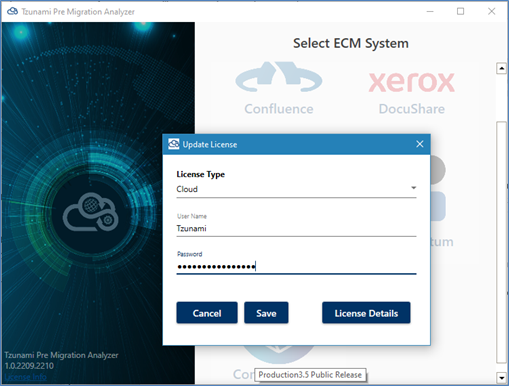
\includegraphics[width=0.8\textwidth]{Images/SelectEcmImage.png}
 \caption{Pre--migration Analyzer License}
\end{figure}
Tzunami Inc may provide the evaluation or full license based on your requirement. The evaluation license has the limitation of 10 items per folder analysis for all feature.
The \appName needs to communicate with Tzunami licensing server. Please, contact with your network administrator if there are any limitation, restriction or proxy environments and contact with Tzunami Support team. \\\\
If you cannot provide connection to Tzunami licensing server, please contact with Tzunami Support team at \href{mailto: sales@tzunami.com}{sales@tzunami.com} and inform with details. Tzunami Support team will contact back to you.

\chapter{GETTING STARTED WITH TZUNAMI PRE-MIGRATION ANALYZER TOOL}
This chapter describes how to create an analysis report using \appName and save analyzed result for future use. This chapter contains the following topics:
\begin{itemize}
  \item Running \appName
  \item Making connection and loading ECM systems
  \item Overview of \appName window Settings for \appName
  \item Generating Report
  \item Analyzing the report generated
  \item Saving and loading, exporting the analyzed report
  \item Features of Analyzer
\end{itemize}
 \section{RUNNING TZUNAMI PRE-MIGRATION ANALYZER REPORT}

\subsection{Running \appName}
\begin{itemize}
\item To run \appName, click Start > All Programs > Tzunami > \appName - for windows 7 or older version, or
For windows 10 and above
Click    button and scroll through the alphabetical list for Tzunami. Under this locate \appName and click it to run. ECM Selection wizard appears as follows:
\begin{figure} 
  \centering
	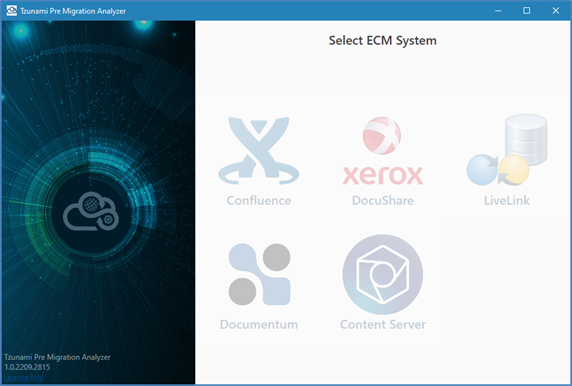
\includegraphics[width=0.8\textwidth]{Images/SelectEccmScreen.png}
 \caption{\appName, Select ECM System screen}
\end{figure}
\item Next select the required ECM system for the Analysis of the source content.
\end{itemize}
Tzunami Inc may provide the evaluation or full license based on your requirement. The evaluation license has the limitation of 10 items per folder analysis for all feature.
The \appName needs to communicate with Tzunami licensing server. Please, contact with your network administrator if there are any limitation, restriction or proxy environments and contact with Tzunami Support team. \\\\
If you cannot provide connection to Tzunami licensing server, please contact with Tzunami Support team at \href{mailto: sales@tzunami.com}{sales@tzunami.com} and inform with details. Tzunami Support team will contact back to you.

\chapter{COPYRIGHT AND TRADEMARK}
© Copyright \the\year{}. \compName All rights reserved.\\ \\
All intellectual property rights in this publication are owned by \compName and protected by the United States copyright laws, other applicable copyright laws and international treaty provisions. \compName retains all rights not expressly granted. No part of this publication may be reproduced in any form whatsoever or used to make any derivative work without prior written approval by \compName
\\ \\
No representation of warranties for fitness for any purpose other than what is specifically stated in this guide is made either by \compName or by its agents.
\\ \\
\compName reserves the right to revise this publication, and/or make improvements or changes in the product(s) and/or the program(s) described in this documentation at any time without prior notice.
\\ \\
Any software on removable media described in this publication is furnished under a license agreement included with the product as a separate document. If you are unable to locate a copy, please contact \compName and a copy will be forwarded to you.
\\ \\
Tzunami is either a registered trademark or a trademark of \compName in the United States and/or other countries.
\\\\
All other brands or product names are trademarks or registered trademarks of their respective companies.
\\ \\
For further information, you can contact \compName at: 
\\
\compName \\
601 108th Avenue, NE \\
Suite 1900\\
Bellevue, WA 98004, USA\\
\href{mailto: sales@tzunami.com}{sales@tzunami.com}
\href{mailto: support@tzunami.com}{support@tzunami.com}\\
\url{http://www.tzunami.com}		
\end{document}
